%&tex
\documentclass{standalone}

\usepackage{graphicx}

\usepackage{cleveref}
\usepackage{subcaption}

\usepackage{tikz}
\usetikzlibrary{arrows,shapes,backgrounds,calc}

\begin{document}


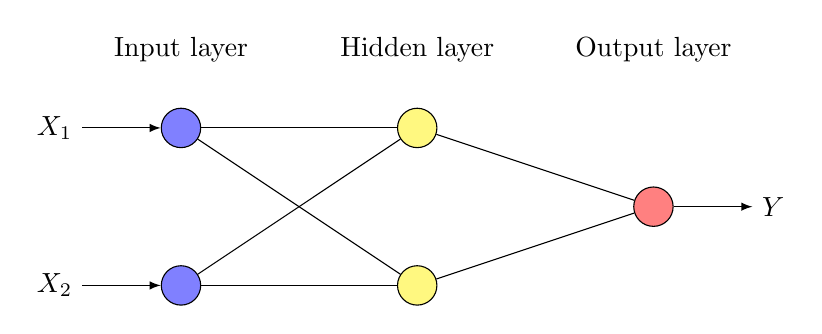
\begin{tikzpicture}

	% input layers
	\node[draw,
	circle,
	minimum size = 0.5cm,
	fill = blue!50] (X1) at (0,1) {};
	\node[draw,
	circle,
	minimum size = 0.5cm,
	fill = blue!50] (X2) at (0,-1) {};

	% hidden layers
	\node[draw,
	circle,
	minimum size = 0.5cm,
	fill = yellow!50] (H1) at (3,1) {};
	\node[draw,
	circle,
	minimum size = 0.5cm,
	fill = yellow!50] (H2) at (3,-1) {};

	% output layer
	\node[draw,
	circle,
	minimum size = 0.5cm,
	fill = red!50] (Y) at (6,0) {};

	% drawing connections
	\draw (X1) -- (H1);
	\draw (X1) -- (H2);
	\draw (X2) -- (H1);
	\draw (X2) -- (H2);
	\draw (H1) -- (Y);
	\draw (H2) -- (Y);
	\draw[latex-] (X1.west) -- ++(-1,0) node[left] {$X_1$};
	\draw[latex-] (X2.west) -- ++(-1,0) node[left] {$X_2$};
	\draw[-latex] (Y.east) -- ++(1,0) node[right] {$Y$};

	% defining labels
	\node at (0,2) {Input layer};
	\node at (3,2) {Hidden layer};
	\node at (6,2) {Output layer};

\end{tikzpicture}

\end{document}
